\chapter{System Architecture}

\section{Architectural View}
WhisperTunnel can be represented as two symmetric endpoint stacks connected by a single authenticated TCP channel. Each endpoint stack has three local layers:

\begin{enumerate}[leftmargin=2em]
\item Interface layer: Linux TUN device receives or emits IP packets.
\item Processing layer: encryption/decryption and framing logic.
\item Transport layer: TCP socket handling and thread-managed I/O.
\end{enumerate}

\begin{figure}[H]
\centering
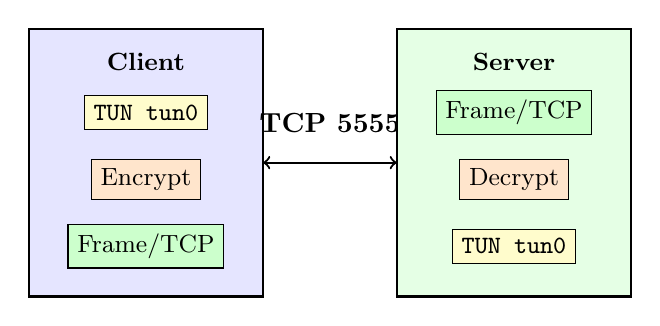
\begin{tikzpicture}[scale=0.85, every node/.style={font=\small}]
  % Client side
  \draw[thick, fill=blue!10] (0,3) rectangle (3.5,7);
  \node at (1.75,6.5) {\textbf{Client}};
  \node[rectangle, draw, fill=yellow!20, minimum height=0.4cm] at (1.75,5.75) {\texttt{TUN tun0}};
  \node[rectangle, draw, fill=orange!20, minimum height=0.4cm] at (1.75,4.75) {Encrypt};
  \node[rectangle, draw, fill=green!20, minimum height=0.4cm] at (1.75,3.75) {Frame/TCP};
  
  % Transport
  \draw[thick, <->] (3.5,5) -- (5.5,5);
  \node[font=\bfseries, above] at (4.5,5.3) {TCP 5555};
  
  % Server side
  \draw[thick, fill=green!10] (5.5,3) rectangle (9,7);
  \node at (7.25,6.5) {\textbf{Server}};
  \node[rectangle, draw, fill=green!20, minimum height=0.4cm] at (7.25,5.75) {Frame/TCP};
  \node[rectangle, draw, fill=orange!20, minimum height=0.4cm] at (7.25,4.75) {Decrypt};
  \node[rectangle, draw, fill=yellow!20, minimum height=0.4cm] at (7.25,3.75) {\texttt{TUN tun0}};
\end{tikzpicture}
\caption{WhisperTunnel System Architecture}
\end{figure}

\section{Lifecycle Sequence}
\subsection{Client}
\begin{enumerate}[leftmargin=2em]
\item Load config and decode base64 key.
\item Establish TCP connection to server.
\item Perform authentication handshake as client.
\item Create and configure \texttt{tun0}.
\item Start two forwarding threads:
  \begin{itemize}[leftmargin=2em]
  \item TUN to socket (encrypt + send).
  \item Socket to TUN (receive + decrypt + inject).
  \end{itemize}
\item Emit periodic stats and handle shutdown signals.
\end{enumerate}

\subsection{Server}
\begin{enumerate}[leftmargin=2em]
\item Load config and decode key.
\item Create and configure \texttt{tun0}.
\item Bind/listen on configured host and port.
\item Accept one client and authenticate.
\item Start forwarding threads equivalent to client directionality.
\item Emit periodic stats, cleanup on termination.
\end{enumerate}

\section{Component Interaction Table}
\begin{table}[H]
\centering
\caption{Primary Runtime Components and Interactions}
\begin{tabular}{p{0.24\textwidth}p{0.30\textwidth}p{0.34\textwidth}}
\toprule
\textbf{Component} & \textbf{Consumes} & \textbf{Produces} \\
\midrule
\texttt{TunInterface} & Kernel-routed IP packets & User-space packet bytes \\
\texttt{encrypt/decrypt} & Plaintext or ciphertext bytes & Ciphertext or plaintext bytes \\
\texttt{PacketFramer} & Byte payloads & Length-delimited stream messages \\
\texttt{authenticate\_connection} & Socket + shared key & Authenticated session state \\
\texttt{Stats} & Packet sizes and error events & Operational counters \\
\bottomrule
\end{tabular}
\end{table}

\section{Threading and Concurrency Model}
Both endpoint processes use a thread-per-direction model for data forwarding. The loops are intentionally simple:

\begin{itemize}[leftmargin=2em]
\item Blocking/timeout I/O keeps CPU usage reasonable.
\item Exceptions break loops and trigger cleanup via \texttt{stop()}.
\item Shared state is small (\texttt{self.running}, sockets, stats counters).
\end{itemize}

This approach is easy to explain and debug but is not the highest-throughput architecture.

\section{Failure Boundaries}
Failure can occur at several boundaries:
\begin{itemize}[leftmargin=2em]
\item Authentication boundary: invalid token or stale timestamp.
\item Crypto boundary: malformed ciphertext, wrong key, tampering.
\item Tunnel boundary: missing privileges or TUN setup failures.
\item Transport boundary: socket disconnects and framing errors.
\end{itemize}

The code responds by logging and exiting loop context, favoring explicit failure over hidden retry complexity.

\section{Representative Flow Snippet}
\begin{lstlisting}[style=vpnpython,caption={Client data-plane pattern (conceptualized from implementation)}]
while self.running:
    packet = self.tun.read_packet(timeout=1.0)
    if packet is None:
        continue
    encrypted = encrypt(packet, self.key)
    self.framer.send(encrypted)
\end{lstlisting}

The mirrored receive path uses \texttt{self.framer.recv()}, then \texttt{decrypt()}, then \texttt{self.tun.write\_packet()}.

\section{Design Trade-Offs}
\begin{table}[H]
\centering
\caption{Notable Trade-Offs}
\begin{tabular}{p{0.30\textwidth}p{0.26\textwidth}p{0.30\textwidth}}
\toprule
\textbf{Decision} & \textbf{Advantage} & \textbf{Cost} \\
\midrule
TCP transport & Simpler reliability/framing model & Added latency, head-of-line blocking \\
Single-client listen(1) & Reduced complexity & No horizontal user scalability \\
Static shared key & Easy setup and deterministic tests & No per-client identity or rotation \\
Threaded loops & Readable control flow & Limited multicore scaling \\
\bottomrule
\end{tabular}
\end{table}

\section{Architecture Integrity Assessment}
Despite MVP constraints, the architecture is coherent:
\begin{itemize}[leftmargin=2em]
\item Responsibilities are mostly localized by module.
\item Packet path is deterministic and auditable.
\item Security controls align with educational scope declarations.
\item Operational scripts bridge theory and runnable environments.
\end{itemize}

The next chapter examines the protocol and cryptography stack in detail, where most correctness and security properties are anchored.
